% fig_phase.tex -- the order-weight profile in the three phases.
% Values are the measured profiles of Table~\ref{tab:profile}.
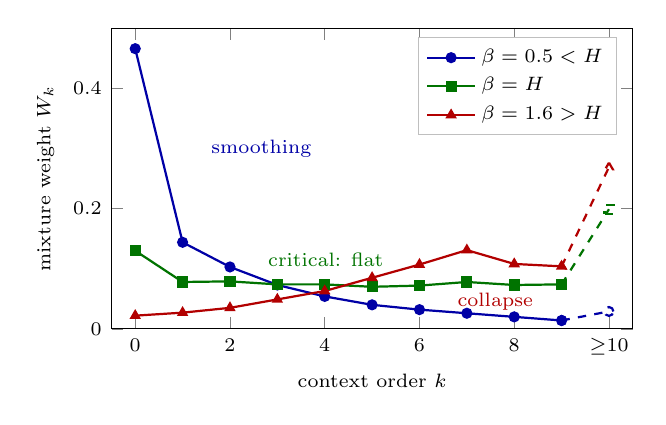
\begin{tikzpicture}
\begin{axis}[width=8.2cm,height=5.4cm,
  xlabel={context order $k$},ylabel={mixture weight $W_k$},
  xmin=-0.5,xmax=10.5,ymin=0,ymax=0.50,
  xtick={0,2,4,6,8,10},
  xticklabels={0,2,4,6,8,$\ge$10},
  legend cell align=left,legend pos=north east,
  legend style={font=\scriptsize,draw=gray!50},
  tick label style={font=\scriptsize},
  label style={font=\scriptsize},
  every axis plot/.append style={thick,mark size=1.6pt}]

% beta = 0.5  (smoothing phase: weight decays with order)
\addplot[blue!65!black,mark=*] coordinates {
  (0,.466)(1,.144)(2,.103)(3,.073)(4,.054)(5,.040)(6,.032)(7,.026)
  (8,.020)(9,.014)};
\addplot[blue!65!black,mark=o,dashed,forget plot]
  coordinates {(9,.014)(10,.029)};

% beta = H  (critical: profile flat)
\addplot[green!45!black,mark=square*] coordinates {
  (0,.130)(1,.078)(2,.079)(3,.074)(4,.074)(5,.070)(6,.072)(7,.078)
  (8,.073)(9,.074)};
\addplot[green!45!black,mark=square,dashed,forget plot]
  coordinates {(9,.074)(10,.199)};

% beta = 1.6  (collapse: weight climbs to the longest match)
\addplot[red!70!black,mark=triangle*] coordinates {
  (0,.022)(1,.027)(2,.035)(3,.049)(4,.063)(5,.085)(6,.107)(7,.131)
  (8,.108)(9,.104)};
\addplot[red!70!black,mark=triangle,dashed,forget plot]
  coordinates {(9,.104)(10,.269)};

\legend{$\beta=0.5<H$,$\beta=H$,$\beta=1.6>H$}

\node[font=\scriptsize,blue!65!black,anchor=west] at (axis cs:1.4,0.30)
  {smoothing};
\node[font=\scriptsize,green!45!black,anchor=west] at (axis cs:2.6,0.115)
  {critical: flat};
\node[font=\scriptsize,red!70!black,anchor=east] at (axis cs:8.6,0.045)
  {collapse};
\end{axis}
\end{tikzpicture}
